\documentclass[lang=en,11pt,a4paper,citestyle=apa,bibstyle=apa]{elegantpaper}

\usepackage{csquotes}
\usepackage{booktabs}
\usepackage{enumitem}
\usepackage{float}
\usepackage{tabularx}
\usepackage{array}
\usepackage{longtable}
\usepackage{colortbl}
\usepackage{ragged2e}
\usepackage{multirow}
\usepackage{tikz}
\usepackage{xurl}
\usetikzlibrary{arrows.meta,fit,positioning}
\newcolumntype{P}[1]{>{\RaggedRight\arraybackslash}p{#1}}
\hypersetup{colorlinks=true,linkcolor=black,citecolor=black,urlcolor=blue}
\urlstyle{same}
\addbibresource{references.bib}
\DeclareLanguageMapping{english}{english-apa}
\newcommand{\deviceLink}[2]{\href{#1}{\textcolor{blue}{#2}}}

\title{Design of Enterprise IoT: Assignment 1b\\[0.4em]
  \large Smart Turtle Breeding System (STBS)}
\author{\vspace{1em}\Large Team 01\vspace{1em}}
\institute{Jinling Institute of Technology}
\date{\today}

\begin{document}

\maketitle

\vspace{9cm}
\begin{center}
  \renewcommand{\arraystretch}{1}
  \begin{tabularx}{0.90\textwidth}{@{}llX@{}}
    \toprule
    \textbf{Student ID} &
    \textbf{Name} &
    \textbf{Preferred Name} \\
    \midrule
    2422441049 & Li Jingru      & Leamon \\
    2422441046 & Rong Yicheng   & Bacon  \\
    2422441050 & Zhang Zhengyan & Paul   \\
    2422441048 & Ye Taohao      & Leaf   \\
    \bottomrule
  \end{tabularx}
\end{center}

\clearpage

\tableofcontents
\clearpage

\section{Task 1: Solution Overview}

The Smart Turtle Breeding System (STBS) serves 20 indoor or semi-closed Chinese soft-shell turtle units. The architecture separates a device layer, a fog layer and a cloud layer. ESP32-C6 devices collect temperature, pH, ammonia, turbidity, level and flow data; local relay, PWM and driver outputs control the heater, valve and water-cycling pump. A Zigbee coordinator connects the wireless device links and food feeder to a Raspberry Pi 5 edge gateway. The IP camera uses Ethernet through the LAN switch, while the router provides the Internet gateway. The Raspberry Pi aggregates, filters and buffers local data, shows a local dashboard through HDMI, and uploads selected information to the IoT cloud platform over MQTT/HTTPS with TLS. Web, mobile and optional analytics applications support remote access, alerts and longer-term analysis \parencite{Prapti2022,Rastegari2023,Munyaev2026}.


\section{Task 2: IoT Devices}

\subsection{Overview and suitability}

The device set follows the connectivity diagram. ESP32-C6 \#1 handles water-environment sensing, while ESP32-C6 \#2 checks tank functionality and connects level and flow feedback to the water-change controls. GPIO/ADC, UART/I2C and Pulse/GPIO are used inside the device layer; Zigbee provides the short wireless links to the coordinator. The heater, valve and water-cycling pump remain under local relay, PWM or driver control. The IP camera uses Ethernet and the food feeder uses Zigbee. This arrangement keeps immediate control local while the Raspberry Pi 5 gateway aggregates, filters and buffers data before cloud upload.

\subsection{IoT Device Profile}

The device profile below identifies the selected field sensors, two ESP32-C6 controllers, actuators, Zigbee food feeder and IP camera. Each row gives the measurable or controllable property, interface, supporting components and design justification. The Raspberry Pi, Zigbee coordinator, switch and router are described in Tasks 3--4.

\begingroup
\scriptsize
\setlength{\tabcolsep}{1pt}
\setlength{\LTleft}{0pt}
\setlength{\LTright}{0pt}
\setlength{\LTcapwidth}{\textwidth}
\setlength{\LTpre}{0pt}
\setlength{\LTpost}{0pt}
\begin{longtable}{|P{0.12\linewidth}|P{0.065\linewidth}|P{0.095\linewidth}|P{0.095\linewidth}|P{0.21\linewidth}|P{0.16\linewidth}|P{0.19\linewidth}|}
\caption{STBS IoT device profile based on the connectivity diagram and official product specifications.}\label{tab:a1b-device-profile}\\
\hline
\rowcolor{gray!20}\textbf{Name} & \textbf{Type} & \textbf{Feature of Interest} & \textbf{Property} & \textbf{Characteristics} & \textbf{Components} & \textbf{Justification}\\
\hline
\endfirsthead
\hline
\rowcolor{gray!20}\textbf{Name} & \textbf{Type} & \textbf{Feature of Interest} & \textbf{Property} & \textbf{Characteristics} & \textbf{Components} & \textbf{Justification}\\
\hline
\endhead
\hline
\multicolumn{7}{r}{\footnotesize Continued on next page}\\
\endfoot
\hline
\endlastfoot
\deviceLink{https://docs.espressif.com/projects/esp-dev-kits/en/latest/esp32c6/esp32-c6-devkitc-1/index.html}{ESP32-C6-DevKitC-1 (\#1 and \#2)} & Controller / device & Each breeding tank & Local sensing, actuation and Zigbee link & ESP32-C6-WROOM-1; IEEE 802.15.4 and Zigbee 3.0; GPIO, 12-bit ADC, UART, I\textsuperscript{2}C, pulse counter and PWM; 3.3 V logic; 8 MB flash. \parencite{EspressifESP32C6DevKitC1} & Two development boards, antennas, USB-C/5 V supplies, relay/driver modules, ADC voltage dividers, GPIO level conditioning and RS-485-to-UART interface & The two controllers are exactly the two device-layer nodes in the diagram: \#1 handles temperature, pH/NH\textsubscript{3}-N and turbidity; \#2 handles level, flow, valve and pump control. The built-in 802.15.4 radio supports the Zigbee path to the coordinator.\\
\hline
\deviceLink{https://wiki.dfrobot.com/dfr0198/}{DFRobot Waterproof DS18B20 Temperature Sensor (DFR0198)} & Sensor & Water in each breeding tank & Water temperature & 3.0--5.5 V; -55--125~$^{\circ}$C usable range; $\pm$0.5~$^{\circ}$C accuracy from -10--85~$^{\circ}$C; 9--12-bit resolution; 1-Wire digital interface; waterproof probe. \parencite{DFRobotDFR0198} & Stainless-steel probe, 1 m cable, pull-up resistor and waterproof cable gland & The 1-Wire signal is a direct GPIO-compatible temperature input for ESP32-C6 \#1 and keeps the temperature path simple and digital.\\
\hline
\deviceLink{https://wiki.dfrobot.com/sen0711/}{DFRobot Water Quality Ammonia Nitrogen \& pH Sensor (SEN0711)} & Sensor & Water in each breeding tank & NH\textsubscript{3}-N, pH and temperature compensation & NH\textsubscript{3}-N 0--100 mg/L; pH 0--14; IP68; 10--30 VDC; RS-485 Modbus-RTU; response time below 30 s; pH and ammonia values are read from the same integrated probe. \parencite{DFRobotSEN0711} & Integrated probe, 5 m cable, 10--30 VDC supply, DFR0845 isolated RS-485-to-UART converter and shielded twisted pair & One product supplies the pH Meter and NH\textsubscript{3}-N Sensor functions drawn separately in the diagram. The converter makes the RS-485 sensor compatible with the ESP32-C6 UART path.\\
\hline
\deviceLink{https://wiki.dfrobot.com/sen0189/}{DFRobot Gravity Analog Turbidity Sensor (SEN0189)} & Sensor & Water in each breeding tank & Relative turbidity & 5 VDC; analog 0--4.5 V or digital threshold output; response below 500 ms; probe tip is immersible but the controller board must remain dry. \parencite{DFRobotSEN0189} & Optical probe, controller board, protective stilling tube, 5 V supply, sealed enclosure and 3.3 V ADC divider & The analog output follows the diagram's GPIO/ADC connection. A dry enclosure and voltage divider are required because the controller board is not waterproof and the output can exceed the ESP32-C6 ADC range.\\
\hline
\deviceLink{https://wiki.dfrobot.com/sen0257}{DFRobot Gravity Analog Water Pressure Sensor (SEN0257)} & Sensor & Water level in each breeding tank & Pressure-derived water level & 5 VDC; 0.5--4.5 V linear output; 0--1.6 MPa range; IP68; 0.5--1\% full-scale accuracy; response below 2 ms. \parencite{DFRobotSEN0257} & Stainless pressure sensor, G1/2-to-G1/4 adapter, pressure tap, 5 V supply and 3.3 V ADC divider & It provides an analog level signal for ESP32-C6 \#2. The pressure tap can be calibrated to tank depth and the voltage divider protects the controller ADC.\\
\hline
\deviceLink{https://www.dfrobot.com/product-1517.html}{DFRobot Gravity Water Flow Sensor (SEN0217 / YF-S201)} & Sensor & Tank inlet and drain pipes & Flow rate and transferred volume & 1--30 L/min; Hall-effect pulse output; 3.5--12 VDC; approximately 450 pulses/L; $\pm$5\% accuracy over the specified operating range. \parencite{DFRobotSEN0217} & Rotor, Hall sensor, 1/2-inch fittings, screened cable and 3.3 V-compatible pulse level conditioning & The pulse output matches the Pulse/GPIO connection in the diagram. Inlet and drain measurements verify pump operation, valve state and bounded water exchange.\\
\hline
\deviceLink{https://www.aqua-medic.de/de/Produkte/Titanium-Heater~p3831}{Aqua Medic Titanium Heater 500 W} & Actuator & Water in each breeding tank & Heat input and water temperature & 500 W; 110--240 VAC; external controller required; titanium element for aquarium use. \parencite{AquaMedicHeater} & Titanium heating element, relay/contactor, RCD, guarded mount, manual isolation and independent over-temperature cut-out & The heater is an electrically powered actuator controlled by a relay or solid-state driver from ESP32-C6 \#1. The independent cut-out remains outside the software control loop.\\
\hline
\deviceLink{https://www.aquael.com/us/products/aquaristics-us/pumps-circulators-us/unipump/}{AQUAEL UNI PUMP 1500} & Actuator & Tank circulation and water-change line & Water circulation and transfer & 220--240 VAC; 19 W; 1400 L/h; maximum head 1.55 m; suitable for submerged or inline operation. \parencite{AquaelPump} & AC electric pump, strainer, check valve, service bypass, RCD, overload protection and relay/contactor & This is the electric water-cycling pump shown in the diagram. It is not battery-powered. ESP32-C6 \#2 operates it through a properly rated relay or contactor, while flow and level feedback verify operation.\\
\hline
\deviceLink{https://www.burkert.com/en/products/solenoid-valves/general-purpose-2-2-solenoids/270895}{Bürkert Type 6213 EV Normally Closed Valve, 24 VDC} & Actuator & Tank inlet and drain lines & Water flow state & Servo-assisted 2/2-way diaphragm valve; normally closed; 24 VDC variant; water service; selected variant rated for the pipe pressure and temperature. \parencite{Burkert6213} & Solenoid coil, flyback suppression, 24 VDC supply, manual isolation, upstream strainer and relay/driver & Normally closed action provides a fail-safe boundary. Level and flow feedback allow ESP32-C6 \#2 to stop a partial water change when the target or a fault condition is reached.\\
\hline
\deviceLink{https://www.aqara.com/en/product/smart-pet-feeder-c1/specs/}{Aqara Smart Pet Feeder C1 (PETC1-M01)} & Actuator / device & Dry feed supplied to each breeding unit & Feeding schedule, portion and feeder status & Zigbee IEEE 802.15.4; 5 V, 1 A USB power; 4 L hopper; feeding statistics in grams; local schedules continue without Internet when powered. \parencite{AqaraPETC1} & Hopper, dispensing motor, portion mechanism, USB power cable, Zigbee radio and local schedule memory & This device directly matches the diagram's Zigbee Food Feeder. Pellet size and portion calibration must be verified for turtle feed before deployment.\\
\hline
\deviceLink{https://support.reolink.com/c/rlc-811a/}{Reolink RLC-811A} & Sensor / device & Turtle activity, feeding and nesting areas & Video and event evidence & 8 MP at up to 25 fps; H.264/H.265; 5$\times$ optical zoom; PoE IEEE 802.3af or 12 VDC; 10/100 Mbps RJ45; RTSP/HTTPS; IP67; microSD support. \parencite{Reolink811A} & Image sensor, lens, processor, PoE/Ethernet interface, mount, privacy mask and local microSD storage & Wired PoE matches the diagram's Ethernet IP camera path. Local recording and selected event/video uploads reduce dependence on continuous cloud video.\\
\hline
\end{longtable}

\endgroup

\section{Task 3: IoT Network Technology}

The network design follows the connectivity diagram exactly: 1-Wire/GPIO connects temperature, RS-485 Modbus through an isolated RS-485-to-UART converter connects the combined pH/NH\textsubscript{3}-N sensor, GPIO/ADC connects the analog turbidity and pressure-level sensors, and Pulse/GPIO connects the flow sensor. Relay/PWM/driver signals control the heater, normally-closed valve and AC electric water-cycling pump. Zigbee at 2.4\,GHz under IEEE 802.15.4 connects the ESP32-C6 nodes and native Zigbee food feeder to the coordinator; Ethernet connects the Reolink camera and fog/network devices; MQTT/HTTPS over TLS connects the gateway to the cloud \parencite{EspressifESP32C6DevKitC1,DFRobotDFR0845}.

\begingroup
\footnotesize
\setlength{\tabcolsep}{1pt}
\setlength{\LTleft}{0pt}
\setlength{\LTright}{0pt}
\setlength{\LTcapwidth}{\textwidth}
\setlength{\LTpre}{0pt}
\setlength{\LTpost}{0pt}
\begin{longtable}{|P{0.15\linewidth}|P{0.17\linewidth}|P{0.22\linewidth}|P{0.43\linewidth}|}
\caption{STBS IoT network connectivity.}\label{tab:a1b-network-connectivity}\\
\hline
\rowcolor{gray!20}\textbf{IoT devices, gateways, routers, etc. to connect} & \textbf{Main considerations} & \textbf{Specific questions} & \textbf{Responses}\\
\hline
\endfirsthead
\hline
\rowcolor{gray!20}\textbf{IoT devices, gateways, routers, etc. to connect} & \textbf{Main considerations} & \textbf{Specific questions} & \textbf{Responses}\\
\hline
\endhead
\hline
\multicolumn{4}{r}{\footnotesize Continued on next page}\\
\endfoot
\hline
\endlastfoot
Selected devices: ESP32-C6 \#1/\#2; field sensors and actuators; Aqara C1 feeder; Reolink camera; Zigbee coordinator; Raspberry Pi 5; monitor; switch; router. & Determine the connectivity between selected IoT devices, gateways, routers, etc. & Why do selected devices need to be connected with each other and to the network? & The water-environment detector connects DFR0198, SEN0711 and SEN0189 to ESP32-C6 \#1. The tank-functionality detector connects SEN0257 and SEN0217 to ESP32-C6 \#2 and drives the valve and AC electric water-cycling pump. The two ESP32-C6 nodes and Aqara C1 food feeder use the Zigbee path to the coordinator, while the Reolink camera uses Ethernet. The Raspberry Pi 5 aggregates local status, camera data and feeding events before forwarding selected information to the cloud.\\
\cline{2-4}
 & Determine communication and network technologies required to support connectivity & What are the range and coverage requirements? & DFR0198 uses 1-Wire/GPIO; SEN0711 uses RS-485 Modbus through the DFR0845 isolated converter to UART; SEN0189 and SEN0257 use analog GPIO/ADC with 3.3 V conditioning; and SEN0217 uses conditioned Hall pulses on GPIO. Zigbee links use 2.4\,GHz IEEE 802.15.4 and are shown as no more than 10\,m from the ESP32-C6 nodes or Aqara feeder to the coordinator. The Reolink camera, Raspberry Pi 5, LAN switch and router use Ethernet over RJ45; HDMI connects the local monitor and USB connects the Zigbee dongle.\\
\cline{3-4}
 &  & What are the power consumption constraints? & The ESP32-C6 controllers, sensors, Zigbee coordinator and Aqara feeder require low-voltage local supplies; the valve uses a 24 VDC supply; the heater and water-cycling pump are mains-powered electrical actuators; and the Reolink camera can use PoE. The pump is not battery-powered. The LAN switch, Raspberry Pi 5, monitor and router require suitable local power. RCD/overload protection and a local backup should preserve the gateway, coordinator and controllers long enough to record alarms and keep bounded local control available.\\
\cline{3-4}
 &  & What is the required data rate (how much data needs to be transmitted over time)? & Temperature, pH/NH3-N, turbidity, level and flow readings, actuator states and Aqara feeder events are low-rate telemetry. The IP camera is the bandwidth-heavy device and therefore uses Ethernet to the LAN switch. The Raspberry Pi 5 aggregates and filters the local streams, so the cloud receives selected telemetry, events or processed video rather than requiring every raw local signal to travel continuously over the Internet.\\
\cline{3-4}
 &  & What are the latency requirements (how fast does data need to be transmitted)? & Heater, valve and AC pump decisions use local relay, PWM or driver signals and do not wait for the cloud. Sensor feedback reaches the ESP32-C6 controllers over 1-Wire/GPIO, RS-485/UART, GPIO/ADC or Pulse/GPIO links. Zigbee and Ethernet support gateway monitoring and event delivery, while MQTT/HTTPS cloud communication is used for reporting and alerts rather than immediate safety action.\\
\cline{3-4}
 &  & What are the security and reliability requirements? & Local control should continue when the router or Internet is unavailable. The Raspberry Pi 5 stores data locally when upload is interrupted and the gateway labels or forwards buffered events after reconnection. MQTT/HTTPS traffic to the cloud uses TLS; Zigbee devices require authenticated joining and coordinator access control; and actuator commands require local bounds and interlocks. RS-485 isolation, ADC protection, GPIO level conditioning, RCD/overload protection, cable glands and waterproof enclosures are required.\\
\cline{3-4}
 &  & What are the cost considerations? & ESP32-C6 nodes and short Zigbee links reduce point-to-point wiring inside the device layer. Ethernet is reserved for the Reolink IP camera and the fixed fog/network path, while one Raspberry Pi 5 provides local aggregation, buffering and display output. The selected sensors require signal conditioning and protected enclosures; the AC pump and heater require correctly rated switching and electrical protection. Cloud storage and analytics can be scaled according to selected uploads.\\
\cline{3-4}
 &  & Which communication/network technologies are selected? & The diagram selects 1-Wire/GPIO for temperature; RS-485 Modbus through DFR0845 and UART for the combined pH/NH3-N sensor; GPIO/ADC for turbidity and pressure-derived level; Pulse/GPIO for flow; Relay/PWM/Driver for heater, valve and AC pump control; Zigbee at 2.4\,GHz under IEEE 802.15.4 for the ESP32-C6 and Aqara feeder links; Ethernet at 10/100/1000 Mbps over RJ45 for the Reolink camera and fog/network path; USB for the coordinator; HDMI for the local monitor; and MQTT/HTTPS over TLS for the Internet connection to the IoT cloud platform.\\
\end{longtable}

\endgroup

\section{Task 4: Fog and Cloud Computing}

The Raspberry Pi 5 is the fog gateway for data aggregation, local control rules, filtering, optional video processing, local buffering and upload to the cloud. The USB Zigbee coordinator bridges the ESP32-C6 and Aqara feeder links to the gateway. The HDMI-connected local monitor is display-only. The router provides the Internet gateway, while the IoT cloud platform supports long-term storage, analytics, notifications, remote access, model training and device management. The cloud is therefore useful for applications and historical analysis but is not placed in the immediate actuator control loop \parencite{RaspberryPi5,SONOFFZBDongleE}.

\begingroup
\footnotesize
\setlength{\tabcolsep}{1pt}
\setlength{\LTleft}{0pt}
\setlength{\LTright}{0pt}
\setlength{\LTcapwidth}{\textwidth}
\setlength{\LTpre}{0pt}
\setlength{\LTpost}{0pt}
\begin{longtable}{|P{0.15\linewidth}|P{0.17\linewidth}|P{0.22\linewidth}|P{0.43\linewidth}|}
\caption{STBS fog and cloud connectivity.}\label{tab:a1b-edge-cloud-connectivity}\\
\hline
\rowcolor{gray!20}\textbf{IoT devices and network devices (e.g., router, hub, gateway, etc.)} & \textbf{Main considerations} & \textbf{Specific questions} & \textbf{Responses}\\
\hline
\endfirsthead
\hline
\rowcolor{gray!20}\textbf{IoT devices and network devices (e.g., router, hub, gateway, etc.)} & \textbf{Main considerations} & \textbf{Specific questions} & \textbf{Responses}\\
\hline
\endhead
\hline
\multicolumn{4}{r}{\footnotesize Continued on next page}\\
\endfoot
\hline
\endlastfoot
Edge/fog devices: ESP32-C6 \#1/\#2; Aqara C1 feeder; SONOFF ZBDongle-E coordinator; Raspberry Pi 5; monitor; switch; router. & Determine the connectivity between IoT devices and network devices in the edge/fog layer & Is an edge/fog layer required? Why? & Yes, because two requirements cannot be met from the cloud: local control has to survive an Internet outage, and 20 continuous video streams are too costly in bandwidth and too sensitive in privacy to send out routinely. A fog layer between the device layer and the cloud follows from those two requirements. The Raspberry Pi 5 provides data aggregation, local control rules, data filtering, optional video processing, local buffering and upload to the cloud. This keeps the system useful when the Internet is unavailable and prevents every local signal from depending on a cloud round trip. The SONOFF coordinator bridges the ESP32-C6 and Aqara Zigbee links to the gateway.\\
\cline{3-4}
 &  & Which network device(s) should handle computing across the edge/fog layer? & The Raspberry Pi 5 is the edge gateway and performs the fog-layer computing. The SONOFF ZBDongle-E acts as the Zigbee 3.0 USB coordinator, the LAN switch forwards Ethernet traffic, the router provides the Internet gateway, and the HDMI-connected local monitor is display-only.\\
\cline{3-4}
 &  & What data is transmitted between the IoT devices and network device(s)? & The ESP32-C6 nodes send temperature, pH, NH3-N, turbidity, water level and flow readings, together with actuator states and food-feeder events. The IP camera sends monitoring video over Ethernet. The Raspberry Pi 5 adds timestamps, device identity, local status and event context before forwarding selected data to the cloud.\\
\cline{3-4}
 &  & What data processing and/or analysis tasks should be performed in the edge/fog layer? & The gateway aggregates sensor readings, applies local control rules, filters noisy or unnecessary data, buffers records during Internet loss and can perform optional video processing. It also correlates sensor feedback with heater, valve, pump and feeder actions so the local dashboard can show whether a commanded operation has produced the expected result.\\
\cline{3-4}
 &  & If the fog connects with a user application, what is the purpose of the connection? & The local monitor receives an HDMI display-only connection from the Raspberry Pi 5 and presents a local dashboard. The dashboard shows current water conditions, actuator states, feeder status, camera or event information and gateway health without requiring the cloud connection to be available.\\
\cline{3-4}
 &  & If the fog connects with a system, what is the purpose of the connection? & The Raspberry Pi 5 connects through the LAN switch and router to the IoT cloud platform. It uploads selected telemetry, events, alerts and optional processed video over MQTT/HTTPS with TLS. The gateway can store data locally and forward buffered records after the Internet connection returns.\\
\hline
Cloud path: Raspberry Pi 5; SONOFF coordinator; router; IoT cloud platform; web dashboard; mobile app; optional analytics. & Determine the connectivity to the cloud & Is a cloud layer required? Why? & A cloud layer is required for the tasks that cannot be held on one local gateway: long-term data storage, analytics and visualisation, alerts, remote access, model training and device management, together with multi-user access and history that survive the loss of the site. It is not required for the immediate relay, PWM or driver control in the device layer, which is why it is kept off the control path.\\
\cline{3-4}
 &  & What data should be transmitted to the cloud, and is it from IoT devices or edge/fog layer devices? & The Raspberry Pi 5 should publish aggregated sensor readings, actuator and feeder states, alarms, gateway health and selected event records. Camera data can be uploaded as selected or processed evidence when the optional analytics function is enabled. Raw local control signals remain at the device and fog layers.\\
\cline{3-4}
 &  & What data processing and/or analysis tasks should be performed in the cloud? & The cloud stores long-term records, provides data analytics and visualisation, issues alert and notification workflows, supports remote access through web or mobile applications, enables behaviour or nesting model training when required, and manages authorised device configuration.\\
\cline{3-4}
 &  & If the cloud connects with a user application, what is the purpose of the connection? & The web dashboard provides farm operators with remote status, historical trends, event records and authorised monitoring functions. The mobile app delivers alerts and notifications so operators can respond when a condition requires attention.\\
\cline{3-4}
 &  & If the cloud connects with a system, what is the purpose of the connection? & The optional data-analytics service receives approved cloud data for longer-term comparison, behaviour or nesting analysis and reporting. Cloud-originated configuration requests must be authenticated and bounded by the local gateway and ESP32-C6 control logic before they can affect an actuator.\\
\end{longtable}

\endgroup

\section{Task 5: Overall Solution Connectivity}

\subsection{Graphical representation}

\begin{figure}[H]
\centering
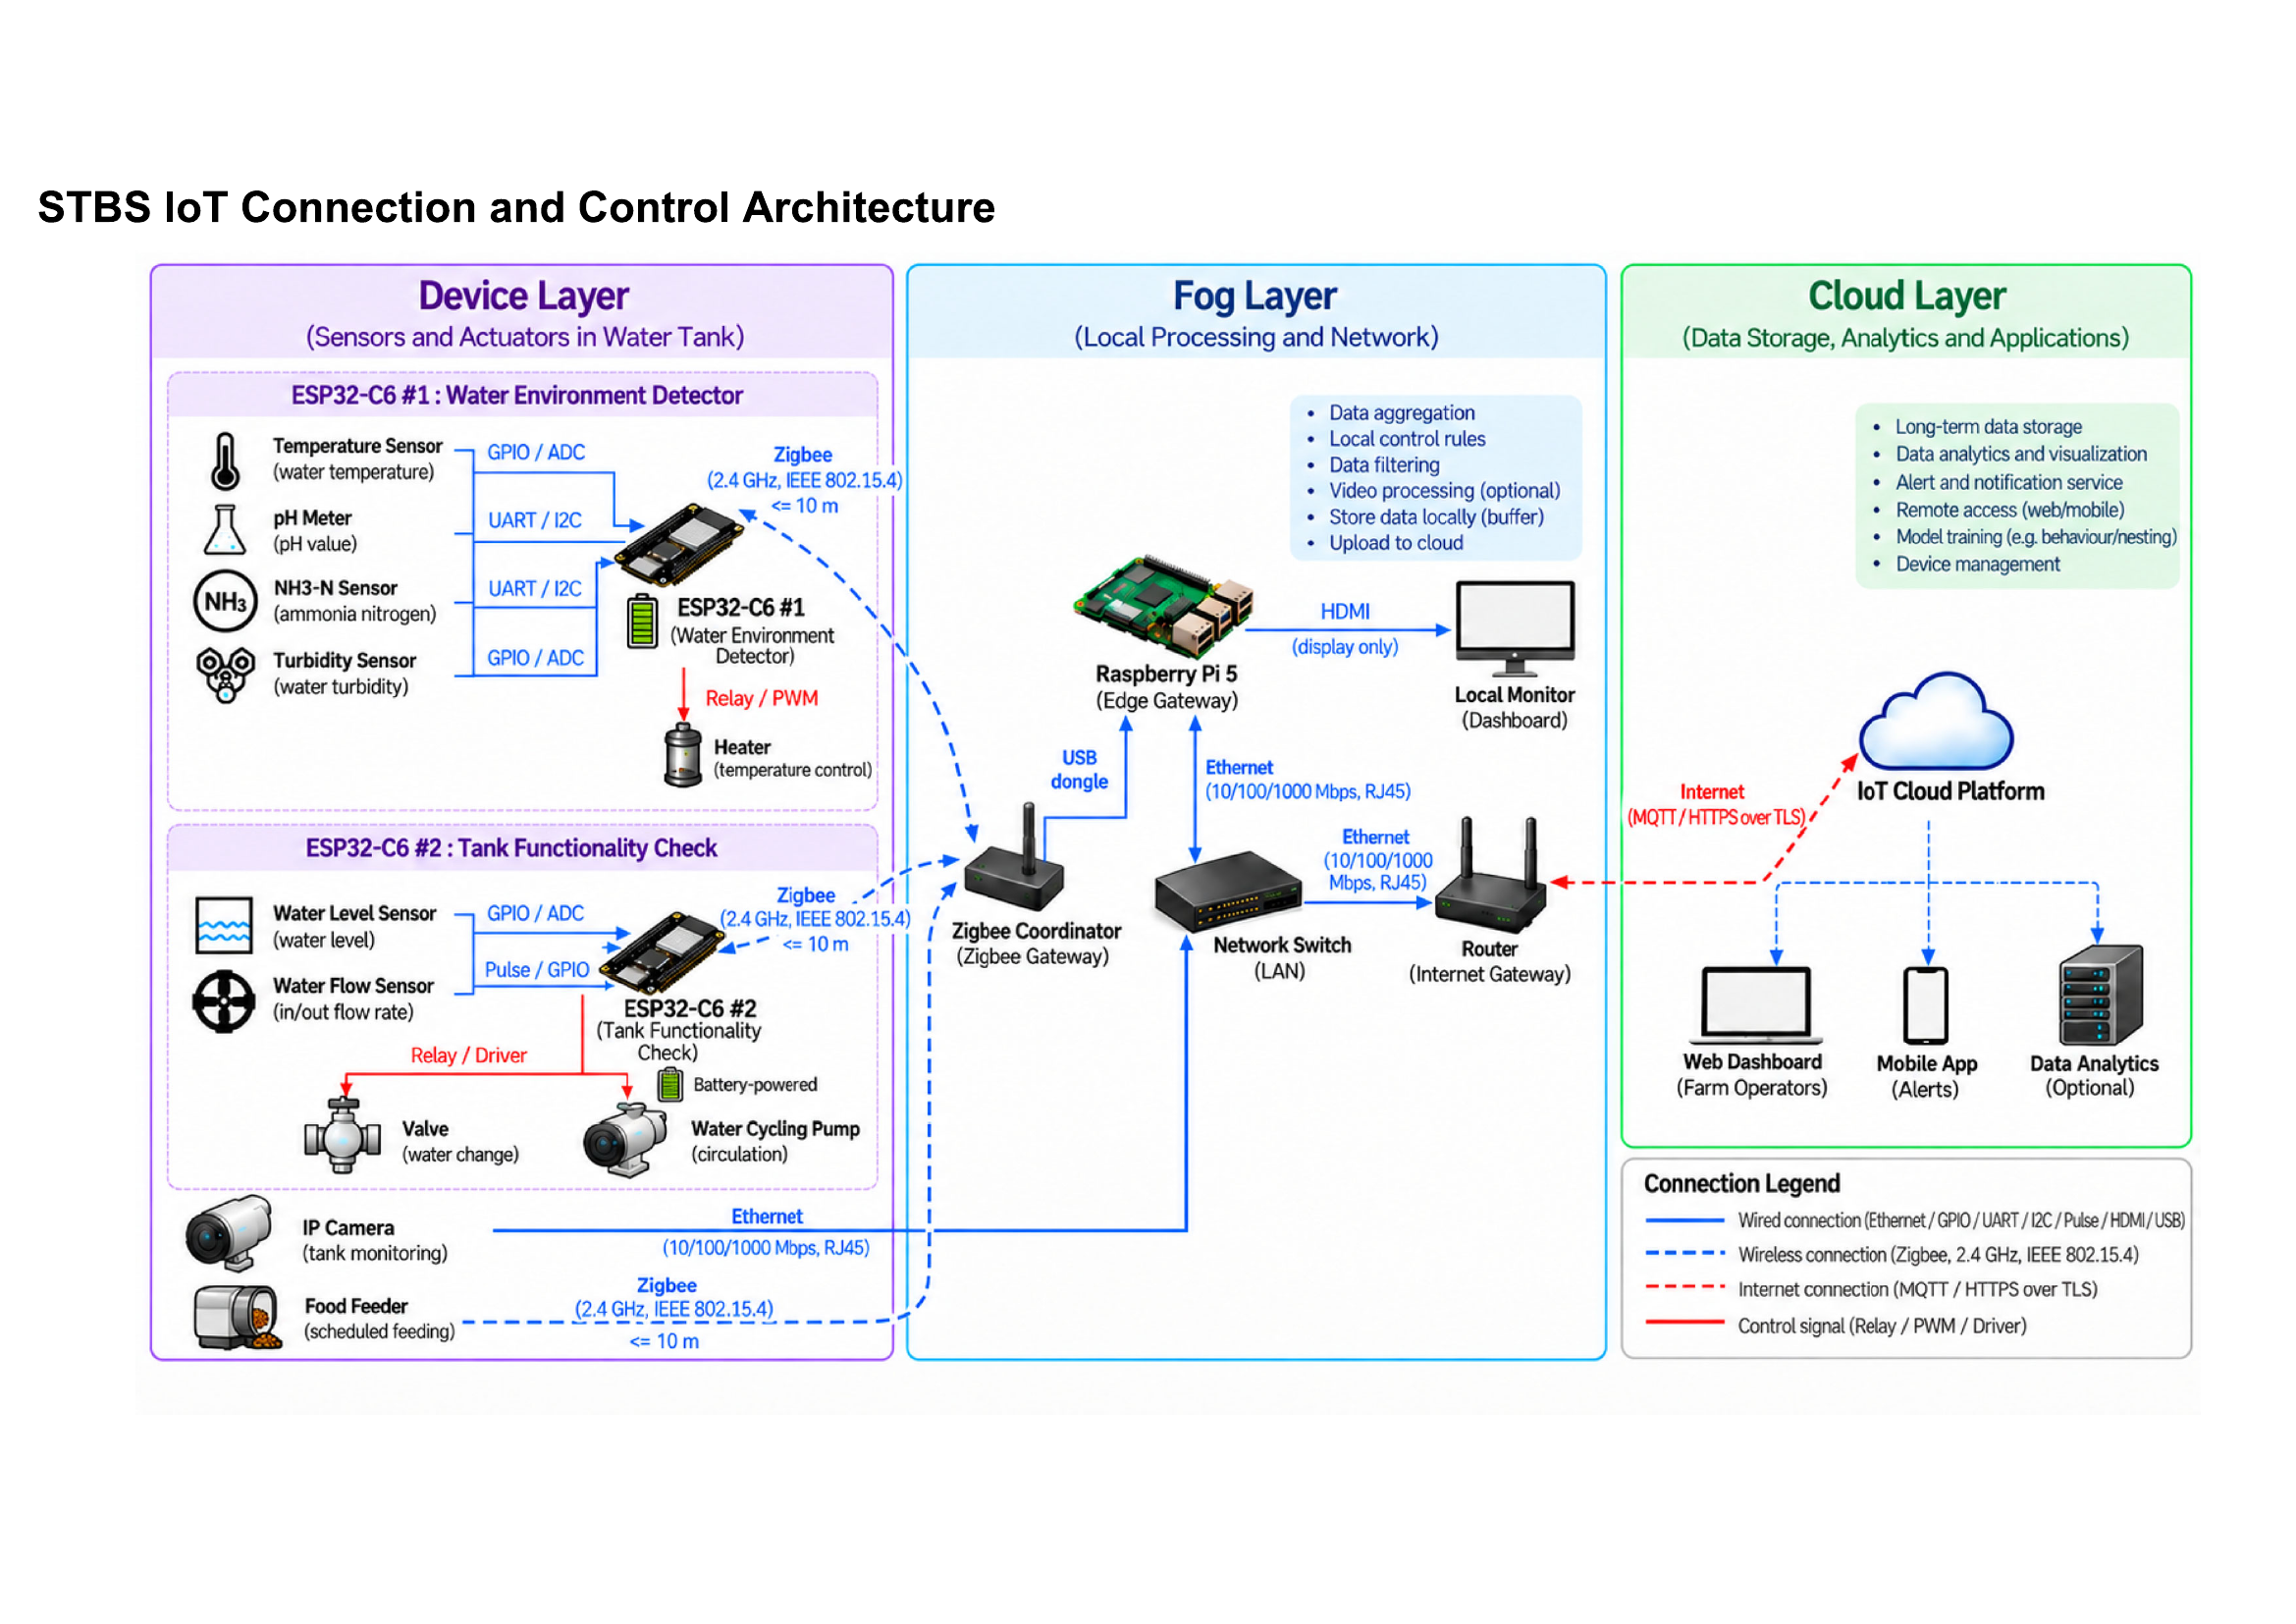
\includegraphics[width=\textwidth,keepaspectratio]{assets/presentation-connectivity-diagram.png}
\caption{STBS connectivity and control architecture.}
\label{fig:architecture}
\end{figure}

\subsection{Description of the diagram}

Figure~\ref{fig:architecture} follows the three-layer structure and connection legend: the device layer senses and actuates, the fog layer aggregates, filters and buffers local data, and the cloud layer stores, analyses and presents authorised results. ESP32-C6 \#1 and \#2 implement the two local device functions, with 1-Wire/GPIO, RS-485/UART, GPIO/ADC and Pulse/GPIO connections to the sensors and relay/PWM/driver outputs to the heater, valve and AC electric pump. The Aqara food feeder is a native Zigbee device; the IP camera uses Ethernet RJ45. The Raspberry Pi 5, USB Zigbee coordinator, switch and router provide the fog/network path, while MQTT/HTTPS over TLS carries selected data to the cloud. Immediate control remains local and does not depend on a cloud round trip.

\section{Task 6: Conclusion}

The design links continuous water and feed measurements, bounded actuation, video evidence and role-specific alerts across 20 units. The diagram keeps immediate sensing and actuation in the device layer, uses Zigbee and Ethernet to connect the local system, and assigns aggregation, filtering and buffering to the Raspberry Pi 5 fog gateway. The water-cycling pump is an AC electric actuator, while the food feeder is a native Zigbee device. The cloud adds long-term storage, visualisation, alerts, remote access and optional behaviour or nesting analytics. The main limitations are probe fouling and calibration effort, wireless range within the 10 m diagrammed Zigbee links, dependence on local gateway and switch power, and the need to validate video models under changing light, water and turtle density. Ammonia and video inference are indicators rather than diagnoses, while feeder runtime only estimates delivered mass. A staged pilot should validate thresholds, wireless coverage, hydraulic timings, electrical protection, false-alarm rates, model performance and operating procedures before all 20 units are commissioned.

\printbibliography[title={References}]

\end{document}
